\section{How it works}
\frame{\frametitle{Agenda} \tableofcontents[currentsection]}
\begin{frame}
\frametitle{Goals and Challenges}
%\begin{columns}
%\column{0.5\textwidth}
\begin{block}{Design Goals}
\begin{itemize}
\item Programmability. Ease of use. 
\item Flexibility. Support various multi/many core processors.
\item High Performance.
\end{itemize}
\end{block}
%\column{0.5\textwidth}
\begin{block}{Challenges}<2->
Result output.
\begin{itemize}
\item Write conflicts among GPU threads.
\item Unknown output buffer size. 
\end{itemize}
\end{block}
\begin{block}{Solution}<3->
\textcolor{red}{Lock-free scheme}
\end{block}
%\end{columns}
\end{frame}

\subsection{Design}

\begin{frame}
\frametitle{Workflow}
\begin{figure}[ht]
\begin{columns}
\column{0.7\textwidth}
\begin{block}{Workflow of Mars}
  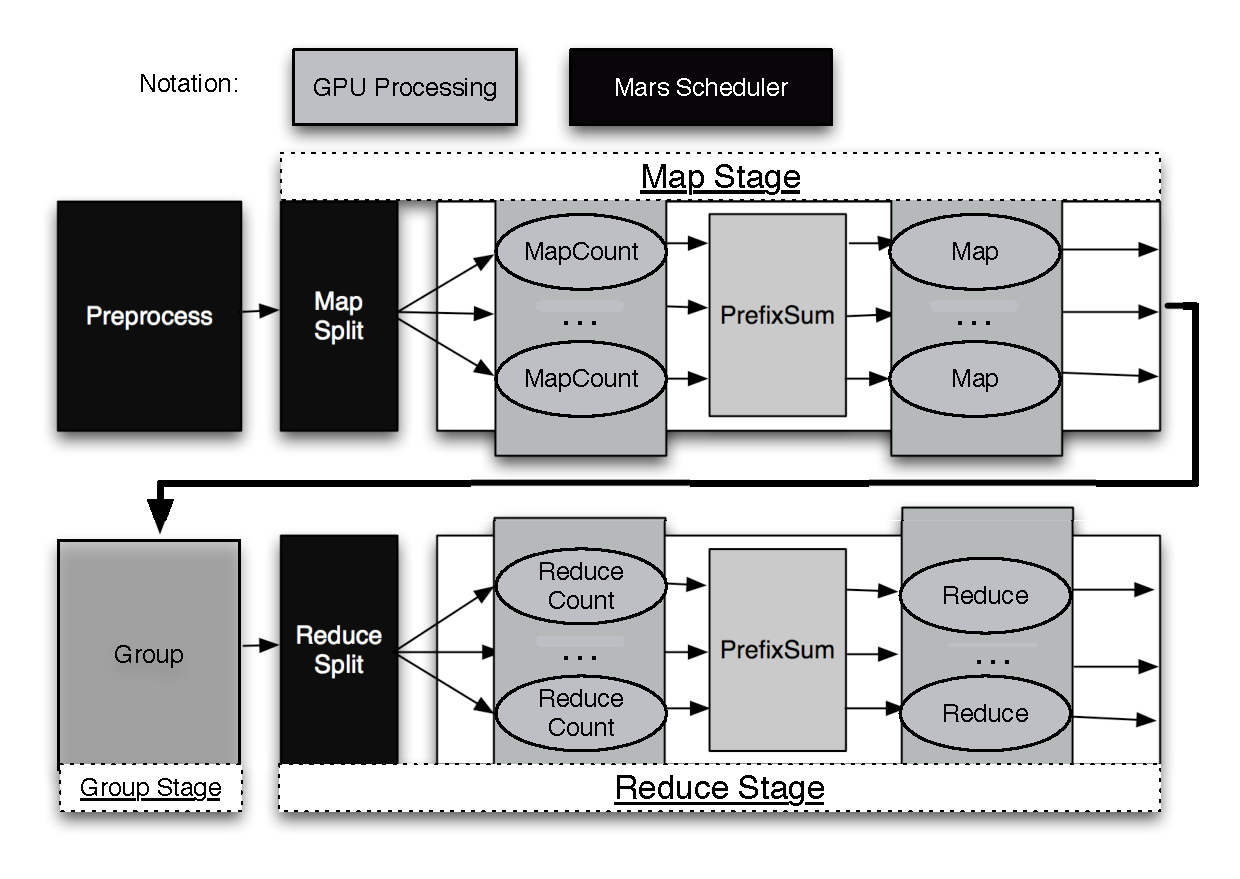
\includegraphics[width=1.00\textwidth]{figure/Mars_workflow.eps}
\end{block}
\column{0.3\textwidth}
\begin{block}{Customizing Workflow}<2->
\begin{itemize}\footnotesize
\item Map Only.
\item Map$\rightarrow$Group.
\item Map$\rightarrow$Group\\$\rightarrow$Reduce.
\item $\cancel{Group\rightarrow Reduce}$.
\item $\cancel{Group}$.
\item $\cancel{Map\rightarrow Reduce}$.
\end{itemize}
\end{block}
\end{columns}
\end{figure}
\end{frame}

\begin{frame}
\frametitle{Data Structure}
\begin{block}{Records}
Input Records $\rightarrow$ \\
\textbf{Map Stage} $\rightarrow$ Intermediate Records I $\rightarrow$ 
\textbf{Group Stage} $\rightarrow$ Intermediate Records II $\rightarrow$ \textbf{Reduce Stage} \\
$\rightarrow$ Output Records
\end{block}
\begin{block}{Structure of Arrays}<2->
\begin{itemize}
\item Key array
\item Value array
\item Directory index array -- Variable-sized record
\begin{itemize}
\item $<$Key size, Key offset, Value size, Value offset$>$
\end{itemize}
\item<3-> Chained MapReduce: \\
Map1$\rightarrow$Group1$\rightarrow$\textcolor{red}{Map2}$\rightarrow$\textcolor{blue}{Map3}$\rightarrow$\textcolor{green}{Map4}$\rightarrow$\textcolor{green}{Group4}
\end{itemize}
\end{block}
\end{frame}


\begin{frame}
\frametitle{Lock-Free Output}
\begin{block}{Lock Free}
\begin{itemize}
\item MapCount
\begin{itemize}
\item Call User defined MapCount function
\item Each function emits intermediate key size and value size
\end{itemize}
\item<2-> Prefix sum on intermediate key sizes and value sizes
\begin{itemize}
\item<2-> The size of intermediate buffer, allocate at one time
\item<2-> The deterministic write position for each Map, lock-free
\end{itemize}
\item<3-> Allocate intermediate buffer
\item<4-> Map
\begin{itemize}
\item<4-> Call User defined Map function
\item<4-> Output records according to the write position
\end{itemize}
\end{itemize}
\end{block}
\end{frame}

\begin{frame}
\frametitle{Lock-Free Output, Example}
\textcolor{red}{Map1 $\rightarrow$ "123456789"}, \textcolor{blue}{Map2 $\rightarrow$ "abcd"}, Map3 $\rightarrow$ "ABCDED" 
\begin{block}{MapCount}<2->
\begin{itemize}
\item \textcolor{red}{MapCount1 $\rightarrow$ 9}
\item \textcolor{blue}{MapCount2 $\rightarrow$ 4}
\item MapCount3 $\rightarrow$ 6
\end{itemize}
\end{block}
\begin{block}{Prefix Sum, Allocate buffer, and Map}<3->
\begin{itemize}
\item<3-> \textcolor{red}{9}, \textcolor{blue}{4},  6 -- size array
\item<4-> \textcolor{red}{0}, \textcolor{blue}{9}, 13 -- write position array
\item<4-> 19 -- output buffer size
\item<5-> Allocate a buffer of size 19
\item<6-> "\textcolor{red}{\underline{1}23456789}\textcolor{blue}{\underline{a}bcd}\underline{A}BCDED"
\end{itemize}
\end{block}
\end{frame}

\subsection{Implementation}
\begin{frame}
\frametitle{MarsCUDA}
\begin{block}{Building blocks}
\begin{itemize}
\item NVIDA CUDA
\item Prefix Sum: CUDPP Library, GPU-based Prefix Sum
\item Group: GPU-based Bitonic Sort
\end{itemize}
\end{block}
\end{frame}

\begin{frame}
\frametitle{MarsCUDA -- Memory Optimization (1)}
\begin{block}{Coalesced Access}
For a half-warp of threads, simultaneous device memory accesses to consecutive device memory addresses can be coalesced into one transaction. $\rightarrow$ Reduce \# of device memory accesses. 
\end{block}
\begin{block}{Local memory}<2->
\begin{itemize}
\item Programmable on-chip memory (shared memory in NVIDIA's term).
\item Exploit local memory in GPU-based Bitonic Sort for Group Stage. 
\item Users can explicitly utilize local memory in their Map/Reduce functions.
\end{itemize}
\end{block}
\end{frame}

\begin{frame}
\frametitle{MarsCUDA -- Memory Optimization (2)}
\begin{block}{Built-in Vector type}
\begin{itemize}
\item Address Alignment
\item {\em float4} and {\em int4}
\item One load instruction to read data of built-in type, of size up to 16 bytes $\rightarrow$ Reduce \# of memory load instructions, compared with reading scalar type
\end{itemize}
\end{block}
\begin{block}{Page-lock host memory}<2->
Prevent OS from paging the locked memory buffer $\rightarrow$ High PCI-E bandwidth
\end{block}
\end{frame}

\begin{frame}
\frametitle{MarsCUDA -- Task distribution}
\begin{block}{Map/Reduce}
$\lceil N/B \rceil$ thread blocks
\begin{itemize}
\item $N$: the number of Map or Reduce tasks
\item $B$: the number of GPU threads per thread block, which is practically set to 256
\item 1 task per GPU thread
\end{itemize}
\end{block}
\begin{block}{Special case for Reduce}<2->
\begin{itemize}
\item Communicative and Associative. For example, Integer Addition.
\item Parallel reduction for load balanced reduce task distribution.
\end{itemize}
\end{block}
\end{frame}


\begin{frame}
\frametitle{MarsCPU}
\begin{block}{Building blocks}
\begin{itemize}
\item pthreads
\item Group: Parallel Merge Sort
\end{itemize}
\end{block}
\begin{block}{General Mars Design}<2->
\begin{itemize}
\item Lock Free
\item $\lceil N/T \rceil$ tasks per CPU thread.
\begin{itemize}
\item $N$: the number of Map or Reduce tasks
\item $T$: the number of CPU threads
\item $N$ is usually much larger than $T$
\end{itemize}
\end{itemize}
\end{block}
\end{frame}

\begin{frame}
\frametitle{GPU/CPU Co-processing}
\begin{figure}[h]
\begin{block}{The workflow of GPU/CPU co-processing}
  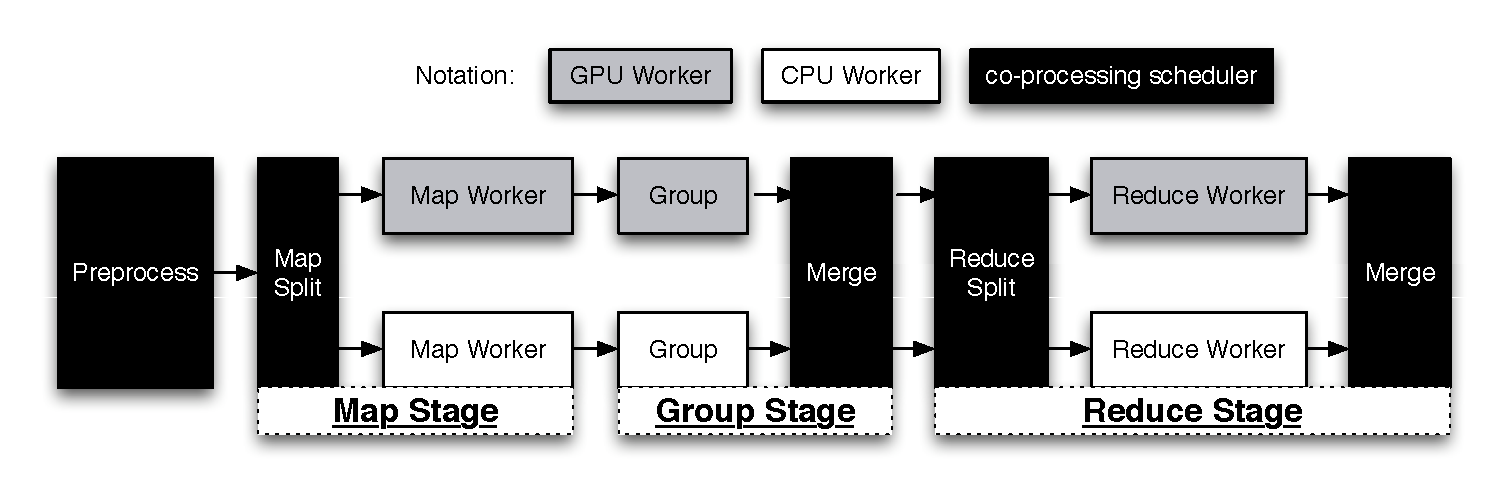
\includegraphics[width=1.00\textwidth]{figure/Mars+.eps} 
\end{block}
\begin{itemize}
\item $I:$ Total size of input data
\item $S:$ Speedup of GPU Worker over CPU Worker
\item Workload for GPU Worker: $\frac{SI}{1+S}$
\item Workload for CPU Worker: $\frac{I}{1+S}$
\end{itemize}
\end{figure}
\end{frame}

\begin{frame}
\frametitle{MarsHadoop}
\begin{figure}[ht]
  \centering
  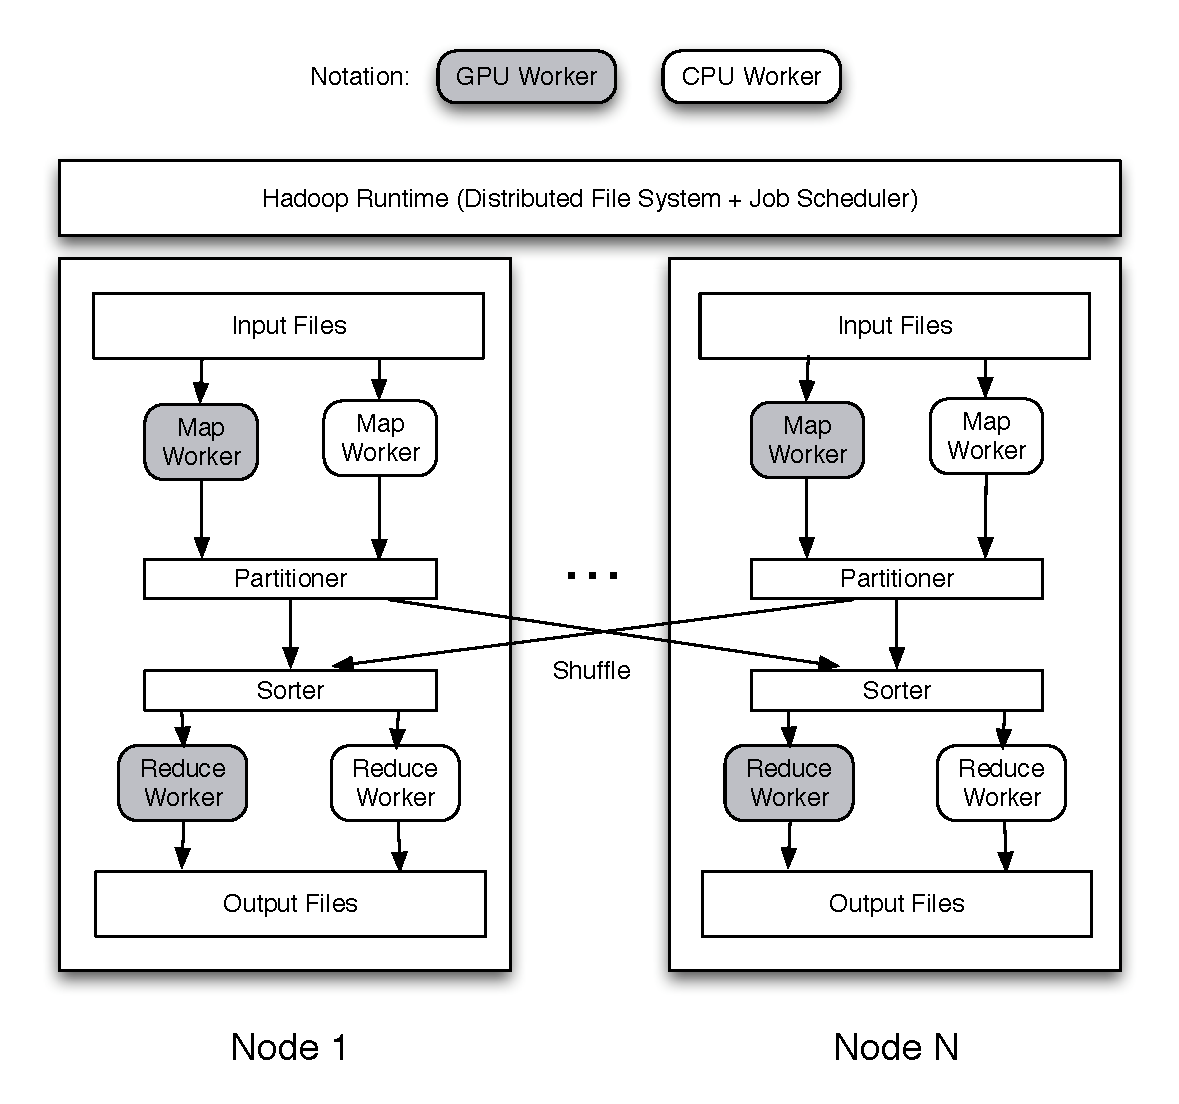
\includegraphics[width=0.62\textwidth]{figure/hadoop.eps} 
  \caption{MarsHadoop. Using {\em Hadoop Streaming}.}\label{fig:hadoop}
\end{figure}
\end{frame}
